\chapter{Introduction}
Neural Machine Translation (NMT) is a radically new way of teaching machines to
translate using deep neural networks. Though developed just last year
\cite{sutskever14,cho14},
NMT has achieved state-of-the-art results in the WMT translation tasks for
various language pairs such as
English-French \cite{luong15}, English-German \cite{jean15,luong15attn}, and
English-Czech \cite{jean15wmt}. NMT is appealing since it is conceptually
simple. NMT is essentially a big recurrent neural network that can be trained
end-to-end and translates as follows. It reads through the given source
words one by one until the
end, and then, starts emitting one target
word at a time until a special end-of-sentence symbol is produced. We illustrate
this process in Figure~\ref{f:nmt}. 
% for the model described in \cite{sutskever14}.

Such simplicity leads to several advantages. 
NMT requires minimal domain knowledge: it only assumes access to
sequences of source and target words as training data and learns to directly
map one into another. NMT beam-search decoders that
generate words from left to right can be easily implemented, unlike the highly
intricate decoders in standard MT \cite{Koehn:2003:SMT}. Lastly, the use of
recurrent neural networks allow NMT to generalize well to very long word
sequences while not having to 
explicitly store any gigantic
phrase tables or language models as in the case of standard MT.
\begin{figure}
\centering
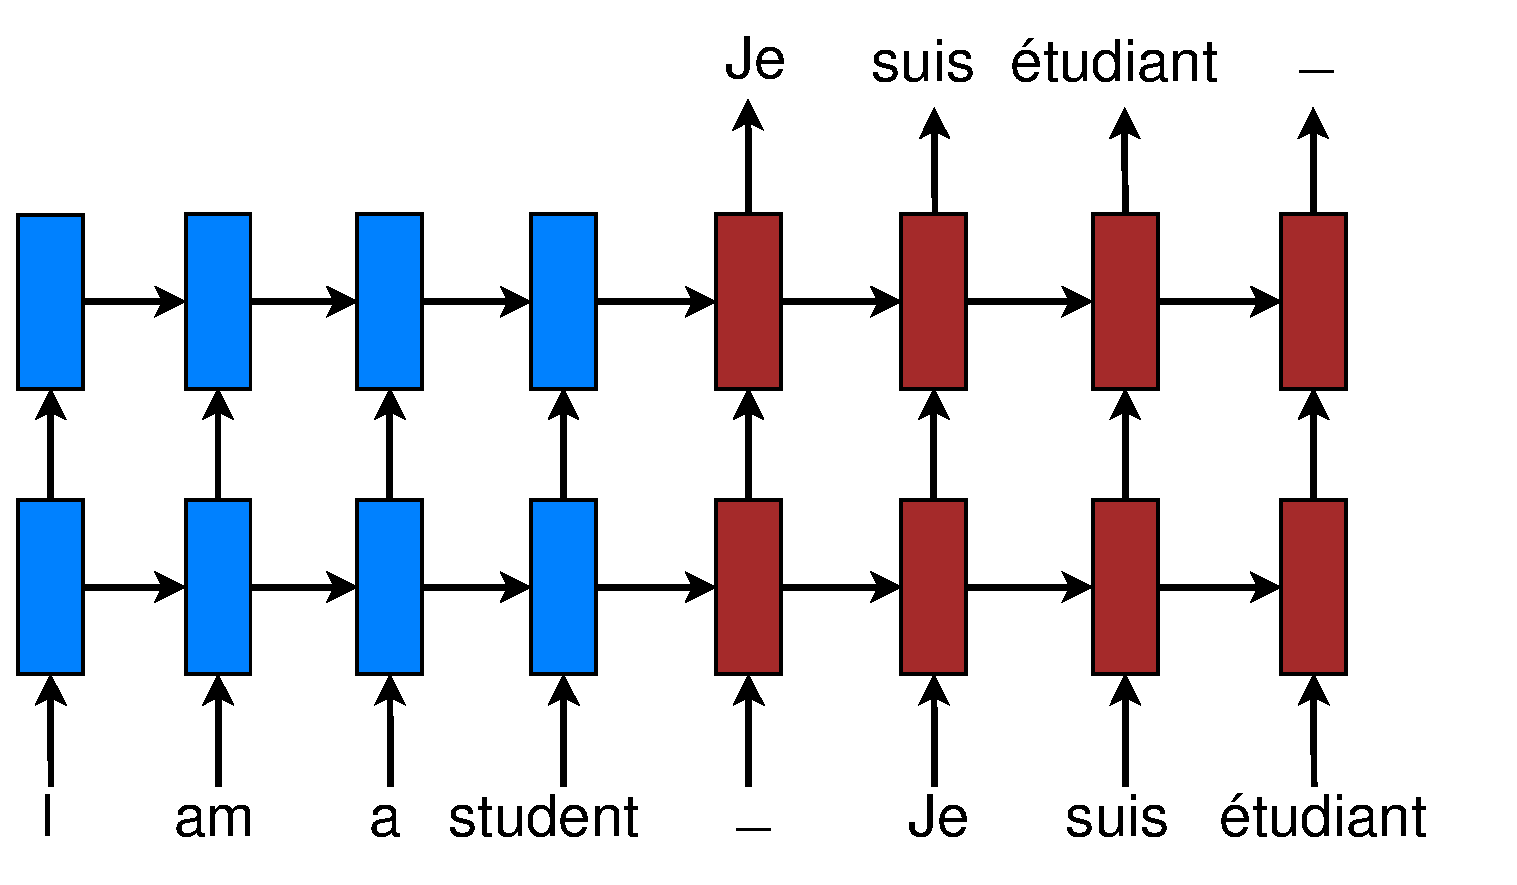
\includegraphics[width=0.45\textwidth, clip=true, trim= 0 0 0 0]{nmt_basic.eps} % , angle=-90
\caption{{\bf Neural machine translation} -- example of a deep recurrent
architecture proposed in \cite{sutskever14} for
translating a source sentence {\it ``I am a student''} into a target sentence
{\it ``Je suis étudiant''}. Here, ``\texttt{\_}'' marks the end of a sentence.
} 
\label{f:nmt}
\end{figure}



Neural Machine Translation (NMT) is a new approach to translating text from one
language into another that captures long-range dependencies in sentences and
generalizes better to unseen texts. The core of NMT is a single deep neural
network with hundreds of millions of neurons that learn to directly map source
sentences to target sentences. Despite being relatively recent, NMT has already
shown promising results on various translation tasks. In this talk, I will
describe how I have pushed the limits of NMT, making it applicable to a wide
variety of languages with state-of-the-art performance. My contributions include
(a) improving the attention mechanism to better select local contexts in the
source sentence, (b) addressing the rare word problem with a "copying"
mechanism, (c) translating at the character level with a hybrid architecture.
Beyond NMT, I will demonstrate how data from a wide variety of tasks such as
translation, parsing, image caption generation, and unsupervised learning can be
jointly utilized.


